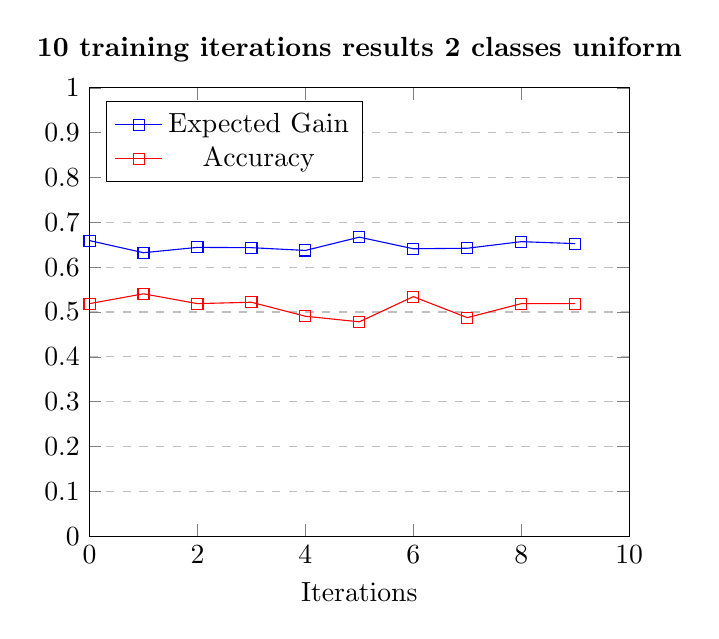
\begin{tikzpicture}
  \begin{axis}[
      title=\textbf{10 training iterations results 2 classes uniform},
      xlabel={Iterations},
      xmin=0, xmax=10,
      ymin=0.0, ymax=1,
      xtick={0,2,4,6,8,10},
      ytick={0.0,0.1,0.2,0.3,0.4,0.5,0.6,0.7,0.8,0.9,1.0},
      legend pos=north west,
      ymajorgrids=true,
      grid style=dashed,
  ]
  
  \addplot[color=blue, mark=square]
    coordinates {
      (0,0.6593504287948415)
      (1,0.6322952653288357)
      (2,0.6442318074145162)
      (3,0.643532034044156)
      (4,0.6374052549173173)
      (5,0.6670332218794528)
      (6,0.641154535217185)
      (7,0.6422862876918007)
      (8,0.6569850006437995)
      (9,0.6526304654809094)
    };
    \addlegendentry{Expected Gain}
  
  \addplot[color=red, mark=square]
    coordinates {
      (0,0.51875)
      (1,0.540625)
      (2,0.51875)
      (3,0.521875)
      (4,0.490625)
      (5,0.478125)
      (6,0.534375)
      (7,0.4875)
      (8,0.51875)
      (9,0.51875)
    };
    \addlegendentry{Accuracy}
      
  \end{axis}
\end{tikzpicture}
